\documentclass[twocolumn]{IEEEtran}

%%\IEEEoverridecommandlockouts

% The preceding line is only needed to identify funding in the first footnote. If that is unneeded, please comment it out.


\usepackage{amsmath,amssymb,amsfonts}

\usepackage{algorithmic}
\usepackage{graphicx}
\graphicspath{ {./images/} }

\usepackage{textcomp}

\usepackage{xcolor}

%\def\BibTeX{{\rm B\kern-.05em{\sc i\kern-.025em b}\kern-.08em

 %   T\kern-.1667em\lower.7ex\hbox{E}\kern-.125emX}}

    \begin{document}



    \title{Parallel Grid Statistics Final Report}

    %{\footnotesize \textsuperscript{*}Note: Sub-titles are not captured in Xplore and

    %should not be used}

    %\%thanks{Identify applicable funding agency here. If none, delete this.}




    \author{\IEEEauthorblockN{1\textsuperscript{st} Nicholas Moran}

    \IEEEauthorblockA{\textit{Computer Science Department} \\

    \textit{University of New Orleans}\\

    New Orleans, LA\\

    nicholas.moran@nrlssc.navy.mil}

    \and

    \IEEEauthorblockN{2\textsuperscript{nd} Norman Schoenhardt}

    \IEEEauthorblockA{\textit{Computer Science Department} \\

    \textit{University of New Orleans}\\

    New Orleans, LA\\

    norman.schoenhardt@nrlssc.navy.mil}

    }


    \maketitle



    \begin{abstract}
        This documents the work preformed on Nicholas Moran, and Norman Schoenhardts Parallel and Scientific Computing class project.
        The projects goal was to create a solution for computing statistics in a fast and simple was for global grid files.

    \end{abstract}



    \begin{IEEEkeywords}

        bathymetry, parallel computing, statistics

    \end{IEEEkeywords}


    \section{Introduction}
There are two predominate methods for predicting global bathymetry in use today.  
The Smith and Sandwell method \cite{sandwell}, and physical collection by survey ships through the use of varying types of sonar.  
The Smith and Sandwell method uses satellite imagery to estimate the mass of seamounts.

\begin{figure}[hb]
    \centering
    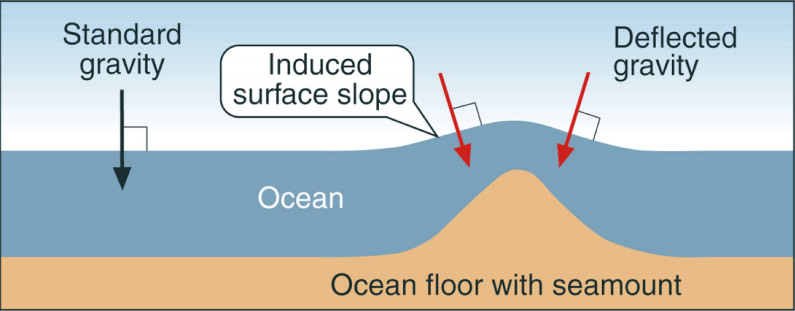
\includegraphics[scale=0.25]{mountainAltimetry}
    \caption{Graphic showing the Smith and Sandwell method}
    \label{fig1:Figure 2}
\end{figure}

\par
This method has known accuracy issues and can be hindered by the presence of clouds and ice formations. 
While not the most accurate solution, satellite calculations provide a mechanism for producing coarse approximations of bathymetry in locations that physical collection is not allowed or ideal. 
The most approximate way to determine bathymetry is through sonar depth soundings. 
Today, ships equipped with sonar, can measure the depth of a given area with great precision.  
While precise, it is not practical to survey the entire globe for bathymetry.  
Constraints to this approach are cost, time, and international law restricting the use of certain maritime areas.

\par
To address these issues the Naval Research Laboratory (NRL) has proposed a research project titled “Predicting Global Altimetry” lead by geophysicist Dr. Warren Wood. 
The goal of this project is to develop models that will accurately predict world-wide bathymetry.  
The method being employed is to use machine learning to train algorithms on different sets of input parameters, for different scenarios, to produce higher resolution bathymetry.  
The input parameters these algorithms require come from multiple sources, but for the scope of this project we will focus on the ones that are calculated from existing datasets.  
It is NRL’s hypothesis that derived statistical data from existing gridded bathymetric data sets can be used as training data to increase prediction accuracy.
    \section{Problem Statement}
This project was created to solve the problem caused by feature extraction on large grids.
High resolution grids are blessed with precise and plentiful data, but cursed by large file sizes.
Extracting features on these requires millions of computations hundreds of computing hours.
However, these extracted features are absolutely required to produce accurate models.
\begin{figure}[h]
    \centering
    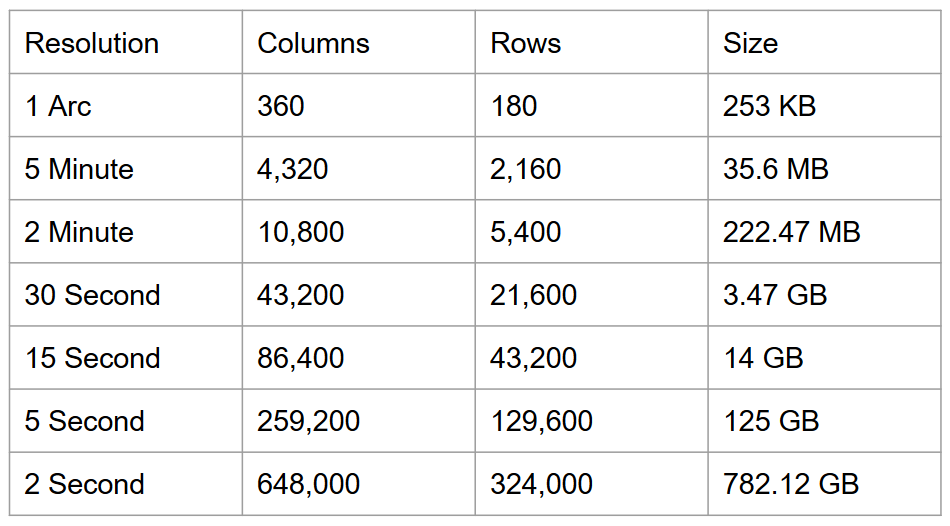
\includegraphics[scale=0.5]{grid_sizes}
    \caption{Graphic showing the sizes of grid files}
  \end{figure}

\par
Programs for extrating these features have been written. 
They were written with fortran, and ran in serial.
The preformance was sufficent for lower resolution grids, but this does not scale to larger grids.
Larger grids require hundreds of hours to complete.
Some statistics scale even worse.
Requiring potentially thousands of hours to compute. 
This leaves a need for quick quick computation.
The size of the grids is also a limiting factor. 
Some of the larger grids require hundreds of gigabytes to represent in memory.

\par
The time complexity for feature extraction effects the ability to test new statistics.
Being able to stream new statistics into models is an efficent way to determine the best features for an accurate model.
This is hindered by the computation time for feature extraction.
New features can not be tested in a model if they have not been computed.
Therefore, the computation bottle neck directly effects the ability to test new models essipically at higher resolutions.

\par
This project needs to solve the following problems.
We need to be able generate new statistics in a time prohibitive mannager.
We also need to create a way to implement new statistics for quick iterative testing with models.
It is also imperative that a solution for handling large grids on a variety of systems is developed.
This will allow our solution to scale up or down.


    \section{Solution}
For this project we developed a parallel framework to abstract out the individual statistical computation components from the parallel implementations. 
The problem we are trying to solve made developing this framework an excellent solution.
When training bathymetric prediction algorithms we do not know in-situ what the ideal features are for optimal prediction. 
Therefore, it is garunteed that we will have to iterate on our statistical computations regularly to improve results. 
Having computation components abstracted from the parallel implementation allows for rapid development and deployment of new statistical computations. 
This allows for more time to train prediction models and evaluate results.

\par
Our solution is comprised of three different implementations, one using OpenMP, one using MPI and one using Java and Java threads. 
It is our hypothesis that each programming paradigm will have strengths and weaknesses for different types of statistical computations. 
In order to find the most efficient use of resources we compared each implementation against a set of statistical computations to determine which performed best. 
We used a 30 second resolution bathymetry grid as our baseline input and used mean, standard deviation and plane fit for the statistical computations.

\par
To address memory consumption with high resolution datasets, we leveraged dynamic memory access. 
Instead of reading an entire grid of data into memory, each process dynamically accesses the memory it needs for computation. 
This approach allowed us to process larger data sets on machines with limited memory. 
When applicable we also leveraged buffered I/O. 
Using buffered I/O limits the amount of disk access when reading data dynamically. 
An example of this can be found in our java implementation. 
Here we used the BufferdReader, BufferedWriter, and FileChannel classes to handle all I/O performed by the computation threads.

    \section{MPI Implementation}
The MPI implementation is another pure C implementation that follows the parallel computational framework we developed. 
The parallel portion of this code relies on the number of processes set at program execution. 
Computation is divided up based on each process being responsible for performing computations on a predetermined number of grid rows. 
MPI\_Bcast was used to share input data across processes and MPI\_Gather was used to receive computation results from each process. 
Individual functions were written to compute mean and standard deviation based on an input grid. 
An integer input parameter was used to signal which type of statistical computation to perform.

\par
The initial design of this implementation was to use a single process to read the input data and use the MPI\_Bcast method to pass the entire grid to each process. 
The though was if each process could contain the entire grid, this would limit the amount of data exchange that would need to take place across active processes. 
However, during execution, the MPI\_Bcast would never complete causing the application to hang. 
We attributed this behavior to the size of the data that was being transmitted.

\par
The second attempt was to let each process read the input grid data. 
While this approach is inefficient, we felt that this was a suitable workaround to the MPI\_Bcast issue. 
This solution was able to process statistical computations but the performance was extremely poor. 
To run the MPI implementation we used the Louisiana Optical Network Infrastructure (LONI) resources. 
LONI sets limitations on the amount of time an application can execute. 
Due to the poor performance of our MPI implementation our processes would be terminated for exceeding these thresholds and a complete output data set would not be generated. 
It is our hypothesis that the large amounts of data being sent between processes, particularly through the MPI\_Gather function, was the cause for the poor performance.

\par
Going forward we would like to develop more sophisticated algorithms that can reduce the amount of data being sent across processes. 
There is potential to preprocess the data by segments using MPI\_Reduce for data that would need to be shared between computing processes. 
This may help to alleviate the amount of message passing needed. 
However, based on our initial findings, distributed memory parallelism does not seem to be well suited for this type of problem.
    \section{OpenMP Implementation}

The first implementation we developed was a pure C based implementation using OpenMP constructs. 
The thought here was to leverage C’s highly efficient computation combined with OpenMP shared memory parallelization. 
The parallel portion of the implementation is comprised of two “for” loops. 
A public outer loop is used to split up grid processing, by rows, across a number of available processes. 
A second private inner loop is then used by each process to iterate over column based computations.

\par
A shared pointer is used for shared reading across processes. 
There are two modes implemented for reading from the input bathymetry grids. 
The first will read the entire grid into memory. 
This mode allows for rapid access to input data but requires a large amount of memory to hold high resolution data grids.  
The second mode uses dynamic buffered reads that allow each process to access the input data as needed. 
The second method was created to test performance on systems with limited amounts of available memory.

\par
We developed an interface for the statistical computations.  
The interface, defined in C header files, contains a single “genStat” function. 
This single entry point into the statistical computation allows for multiple implementations to be developed without having to modify the parallel portion of the code. 
Each statistical computation module can be swapped in and out at compilation time by the inclusion of different header files. 
We implemented two versions of the “genStat” function, one to compute mean, the other to compute standard deviation. 
Due to time restrictions of this class project we were not able to implement a planar regression function in C but plan to do so going forward. 
    \section{Java Implementation}

We implemented a Java threads version of the framework.
This is a pure Java implementation that fully supports all aspects of the framework.
All grids are written in parallel which is a improvement over the C implementation.

\par
Java's executor service is utilized for parallelization.
A main loop runs using the apache commons CLI interface to read inputs and settings.
The main loop then intelligently divides the work and submits each thread to be executed by the executor service.
The executor services will preform the computations on the maximum amount of cores available.

\par
The NIO (Non-Blocking Input/Output) package is used for concurrent writting and reading of grids.
Essentially, a shared object is passed to each process that gives conccurent read access to the grid.
A writer object is used to queue writes to output files.
This queue is able to write to the output file in a non sequential manner by growing the grid file size in-situ.
This is enabled by the NIO FileChannel class by passing the bytes as a stream to the files or processes.

\par
This implementation uses Java interfaces to define the API.
There are 2 main classes defined in the API.
A Generator and a Collector class.
The generator class is implemented to read a grid and calculate a correponding statistic grid.
Generators need to be thread safe and have all statistics submitted to a collector.
A collector class is implemented to handle generated statistics.
Collector's pipe statistics to a generated file.
This piping needs to be implemented in a non-sequential manner.

\par
There are three modules implemented for the Java framework.
There is a mean, standard deviation, and plane fit module implemented.
The plane fit statistic is implemented using the Plane class from the apache commons math package.
A plane fit can be a very computationally exspensive.
The apache commons plane class does a partial fit that is accurate enough and very fast.
This makes it ideal for fitting accurate planes in a efficent amount of time.

\par
This implementation offers a helpful CLI interface that makes running streamlined.
Allowing a user to specify settings, input, and output grids without recompiling.
This makes the Java implementation the most convient version to use.
Currently, the Java implementation is being used to generate grids for the project.

    \section{Results}
For testing the three implementations we used a 30 second bathymetry grid as the baseline input dataset. 
Execution times were recorded by using each programming paradigm’s underlying method for getting current time at application start and application end, subtracting these values and converting to hours. 
From prior work done in the past we had access to a single threaded Fortran program that computes mean and standard deviation for gridded data.  
We used the Fortran execution times previously previously recorded for 30 second input data to compare against our results.  
While not an ideal comparison, time constraints prevented us from creating single threaded versions of our implementations and running them.  
They simply take too long to process a data set as large as the 30 second resolution grid that we used as our baseline.

\par
The Mean and Standard deviation times are shown in Figure 3.
All results were timed in hours for each coresponding core ammount.
As to be expected, the mean and standard deviation graphs fit the classical parallel efficency curve \cite{buzbee}.
Figure 3 does not include results for the MPI implementation because of the impediments discussed earlier in the report.
\begin{figure}[h]
    \centering
    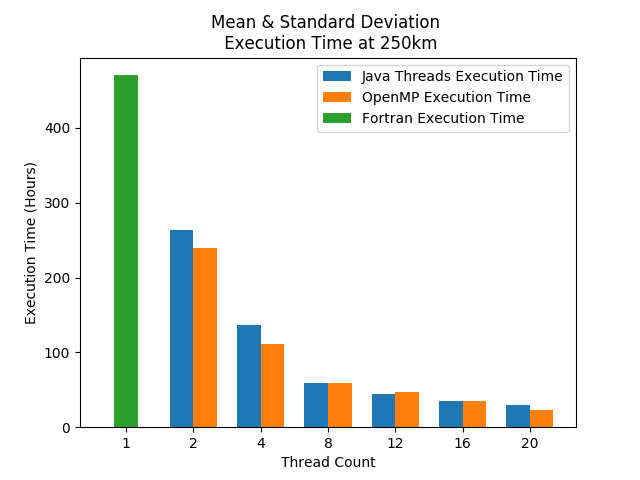
\includegraphics[scale=0.5]{merp}
    \caption{Results for Mean and Standard Deviation}
    \label{fig:3}
\end{figure}

\par
Java threads preformed marginally slower than the C implementation.
However, this slow down scaled as more cores are used in computation.
Going from several days to only several hours at higher core counts.


\par
The Plane fit execution times are shown in Figure 4.
The original Fortran program required months to run.
However, we timed the Java implementation at around two weeks for 20 cores.
We did not run it at lower core counts for lack of time.
Predicting based on a classic parallel computing trend line, the time requirements will be several months to compute those results.

\begin{figure}[h]
    \centering
    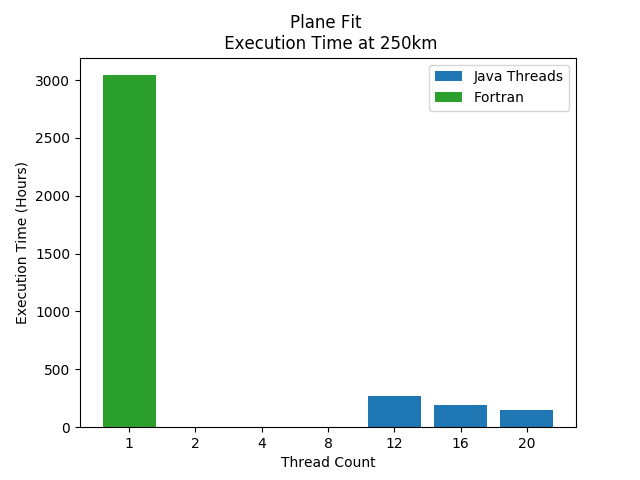
\includegraphics[scale=0.5]{plane}
    \caption{Results for Plane Fit}
    \label{fig:4}
\end{figure}






\end{document}
